\documentclass[12pt]{article}
\usepackage[a4paper, total={6in, 8in}]{geometry}
\usepackage[utf8]{inputenc}
\usepackage{fontenc}
\usepackage{amssymb}
\usepackage{mathrsfs}
\usepackage{amsmath}
\usepackage{graphicx}
\usepackage{setspace}
\singlespacing




\title{\emph{Chapter2:Electromagnetic Waves and Photons}}
\author{Yijie Chen}
\date{}


\numberwithin{equation}{section}
\begin{document}
\maketitle
\tableofcontents
\newpage
\section{Electromagnetism}
All known observations of classical electromagnetism can be explained with the set of equations collectively known as \emph{Maxwell's equations}.
These equations are expressed using Faraday's concept of \emph{electric and magnetic fields} that ultimately become the framework for our description of electromagnetic waves.\\
\indent The \emph{electric field} $\vec{E}$ at a point is defined as the force per unit charge experienced by a \emph{small positive test charge} placed at that point.
Thus, any real charge $q$ will experience a force $\vec{F}=q\,\vec{E}$ when placed within an electric field $\vec{E}$.
The \emph{magnetic field} $\vec{B}$ is also defined in terms of a force; however, the charge $q$ must be moving in order for a magnetic force to act:$\vec{F}=q\vec{v}\times \vec{B}$.
The combination of the electric and magnetic force is called the \emph{Lorentz force}:
\begin{equation}
    \vec{F}=q\,\vec{E}+q\,\vec{v}\times \vec{B}
\end{equation}
The Lorentz force can be taken as the definition of electric and magnetic fields.
\subsection{Gauss's Law for Electric Fields}
\emph{The outward electric flux integrated over a closed surface is proportional to the net electric charge enclosed by the surface.Electric flux} through a \emph{closed surface} is a mathematical concept that can be intuitively visualized with electric field lines.
\emph{Outward electric flux} is defined so that field lines \emph{leaving} the closed surface contribute positively while field lines entering the closed surface contribute negatively.
The contribution to the total electric flux over an infinitesimally small area is $d\,\Phi_E=\vec{E}\cdot \hat{n}\,d\,A $, where $\hat{n}$ is the \emph{outward unit normal} to the surface at the position of $d\,A$.It is customary to define $d\,\vec{A}\equiv \hat{n}\,d\,A$.
According to Gauss:
\begin{equation}
    \Phi_E=\oint_A \vec{E}\cdot d\,\vec{A}=\frac{q_{net}}{\varepsilon_0}=\frac{1}{\varepsilon_0}\int_V \rho \,d\,V\label{12}
\end{equation}
where A is a closed surface,V is the volume enclosed by A, $q_{net}$ is the algebraic sum of all charges contained in V, $\rho$ is the charge per unit volume(charge distribution) within V, and $\varepsilon_{0}$ is the permittivity of free space 
\begin{equation}
    \varepsilon_{0}=8.854\times 10^{-12}\frac{C^2}{Nm^2}
\end{equation}
\newpage
\subsection{Gauss's Law for Magnetic Fields}
\emph{The outward magnetic flux integrated over a closed surface is zero}.This is a statement of the interesting empirical fact that magnetic charges(\emph{magnetic monopoles}) have never been observed.Thus,
\begin{equation}
    \Phi_{M}=\oint_A \vec{B} \cdot d\,\vec{A}=0\label{14}
\end{equation}
\subsection{Faraday's Law of Induction}
\emph{A changing magnetic field induces an electric field}. For a curve C that bounds an area A, Faraday's law is stated as follows:
\begin{equation}
    \oint_C \vec{E}\cdot d\,\vec{l}=-\frac{d}{dt}\int_A \vec{B}\cdot d\,\vec{A}\label{15}
\end{equation}
The minus sign on the right-hand side of Faraday's law is an expression of \emph{Lenz's Law},
which states that currents flowing in response to the induced \emph{electromotive force} produce magnetic fields
oriented so as to \emph{oppose the change} in magnetic flux.\\
The time derivative in Faraday's law may be moved inside the integral sign as a partial derivative:
\begin{equation}
    \oint_C \vec{E}\cdot d\,\vec{l}=-\int_A \frac{\partial{\vec{B}}}{\partial{t}}\,\cdot d\,\vec{A}\label{16}
\end{equation}
\subsection{Ampere's Circuital Law}
\emph{A changing electric field induces a magnetic field.} Ampere's original version of this law was restated by Maxwell to include a displacement current:
\[
    \oint_C \vec{B} \cdot d\,\vec{l}=\mu\,I+\mu(\int_A \epsilon \frac{\partial{\vec{E}}}{\partial{t}}\cdot d\,\vec{A}) 
\]
As in Faraday's law,C bounds A.The symbol $I$ represents the flux of free charge through A:
\[
    \oint_C \vec{B} \cdot d\,\vec{l}=\mu (\int_A \vec{J} \cdot d\,\vec{A})+\mu (\int_A \epsilon \frac{\partial{\vec{E}}}{\partial{t}}\cdot d\,\vec{A})
\]
For \emph{linear,isotropic magnetic materials}, $\mu=K_M\mu_0$, where $K_M$ is the relative permeability and $\mu_0$ is permeability of free space:
\begin{equation}
    \mu_0=4\pi\times10^{-7}\,\frac{T_m}{A}
\end{equation}
For non-magnetic materials, $K_M=1$. In this text, \emph{we assume that all optical materials of interest are non-magnetic}. In this case, $K_M=1$, $\mu=\mu_0$, and Ampere's law becomes
\begin{equation}
    \oint_C \vec{B} \cdot d\,\vec{l}=\mu_0\,I+\mu_0(\int_A \epsilon \frac{\partial{\vec{E}}}{\partial{t}}\cdot d\,\vec{A})\label{18}
\end{equation} 
\indent We will be primarily concerned with regions of space that contain no free charge distributions and no free currents. In this case, Maxwell's equations become:
\begin{equation}
    \oint_A \vec{E}\cdot d\,\vec{A}=0
\end{equation}
\begin{equation}
    \oint_A \vec{B}\cdot d\,\vec{A}=0
\end{equation}
\begin{equation}
    \oint_C \vec{E}\cdot d\,\vec{l}=-\int_A \frac{\partial{\vec{B}}}{\partial{t}}\,\cdot d\,\vec{A}
\end{equation}
\begin{equation}
    \oint_C \vec{B} \cdot d\,\vec{l}=\mu_0\epsilon\int_A \frac{\partial{\vec{E}}}{\partial{t}}\cdot d\,\vec{A}
\end{equation}



\subsection{Example}
\newpage
\section{Electromagnetic Wave Equation}
In this section, we deduce the properties of electromagnetic waves from Maxwell's equations.
We have learned Maxwell's equations in \emph{integral form} in previously section. To find the properties of
electromagnetic waves, we must derive the \emph{differential wave equation for electromagnetic waves}. This is done in the
Appendix at the end of this chapter. The results are summarized below:\\
\indent Faraday's law:

\[
    \frac{\partial{E_y}}{\partial{x}}-\frac{\partial{E_x}}{\partial{y}}=-\frac{\partial{B_z}}{\partial{t}}
\]

\[
    \frac{\partial{E_x}}{\partial{z}}-\frac{\partial{E_z}}{\partial{x}}=-\frac{\partial{B_y}}{\partial{t}}
\]

\[
    \frac{\partial{E_z}}{\partial{y}}-\frac{\partial{E_y}}{\partial{z}}=-\frac{\partial{B_x}}{\partial{t}}
\]
\indent Ampere's law:

\[
    \frac{\partial{B_y}}{\partial{x}}-\frac{\partial{B_x}}{\partial{y}}=\mu_0\,\epsilon\,\,\frac{\partial{E_z}}{\partial{t}}
\]

\[
    \frac{\partial{B_x}}{\partial{z}}-\frac{\partial{B_z}}{\partial{x}}=\mu_0\,\epsilon\,\,\frac{\partial{E_y}}{\partial{t}}
\]  

\[
    \frac{\partial{B_z}}{\partial{y}}-\frac{\partial{B_y}}{\partial{z}}=\mu_0\,\epsilon\,\,\frac{\partial{E_x}}{\partial{t}}
\]

\indent Gauss's law for $\vec{E}$ and $\vec{B}$:

\[
    \frac{\partial{E_x}}{\partial{x}}+\frac{\partial{E_y}}{\partial{y}}+\frac{\partial{E_z}}{\partial{z}}=0
\]

\[
    \frac{\partial{B_x}}{\partial{x}}+\frac{\partial{B_y}}{\partial{y}}+\frac{\partial{B_z}}{\partial{z}}=0
\]
\subsection{Three-dim wave equations}
Let's recall the wave function using \emph{laplacian operator $\nabla^2$}:
\[
    \nabla^2 \Psi(x,y,z,t)=\frac{1}{v^2}\frac{\partial^2{\Psi(x,y,z,t)}}{\partial{t^2}}
\]
Then, we can represent electric field form and magnetic field form:
\[
    \nabla^2 \Psi_E(x,y,z,t)=\frac{1}{v^2}\frac{\partial^2{\Psi_E(x,y,z,t)}}{\partial{t^2}}
\]

\[
    \nabla^2 \Psi_B(x,y,z,t)=\frac{1}{v^2}\frac{\partial^2{\Psi_B(x,y,z,t)}}{\partial{t^2}}
\]
The differential wave equation for $\vec{E}$ is obtained for Cartesian coordinates as follows.
\[
\begin{split}  
    \mu_0\,\epsilon\,\,\frac{\partial^2{E_x}}{\partial{t^2}}=&\frac{\partial}{\partial{t}}\Bigl(\frac{\partial{B_z}}{\partial{y}}-\frac{\partial{B_y}}{\partial{z}}\Bigl)=\frac{\partial}{\partial{y}}\Bigl(\frac{\partial{B_z}}{\partial{t}}\Bigl)-\frac{\partial}{\partial{z}}\Bigl(\frac{\partial{B_y}}{\partial{t}}\Bigl)\\
    \\
    =&\frac{\partial}{\partial{y}}\Bigl(\frac{\partial{E_x}}{\partial{y}}-\frac{\partial{E_y}}{\partial{x}}\Bigl)-\frac{\partial}{\partial{z}}\Bigl(\frac{\partial{E_z}}{\partial{x}}-\frac{\partial{E_x}}{\partial{z}}\Bigl)\\
    \\
    =&\frac{\partial^2{E_x}}{\partial{y^2}}+\frac{\partial^2{E_x}}{\partial{z^2}}-\frac{\partial}{\partial{x}}\Bigl(\frac{\partial{E_y}}{\partial{y}}+\frac{\partial{E_z}}{\partial{z}}\Bigl)\\
    \\
    =&\frac{\partial^2{E_x}}{\partial{y^2}}+\frac{\partial^2{E_x}}{\partial{z^2}}+\frac{\partial^2{E_x}}{\partial{x^2}}-\frac{\partial}{\partial{x}}\Bigl(\frac{\partial{E_y}}{\partial{y}}+\frac{\partial{E_z}}{\partial{z}}\Bigl)-\frac{\partial^2{E_x}}{\partial{x^2}}\\
    \\
    =&\nabla^2{E_x}-\frac{\partial}{\partial{x}}\Bigl(\frac{\partial{E_y}}{\partial{y}}+\frac{\partial{E_z}}{\partial{z}}+\frac{\partial{E_x}}{\partial{x}}\Bigl)
\end{split}
\]
We ignore last term of equation according to \emph{Gauss's law for $\vec{E}$ and $\vec{B}$},
\[
    \mu_0\,\epsilon\,\,\frac{\partial^2{E_x}}{\partial{t^2}}=\nabla^2{E_x}
\]
Generally,
\begin{equation}
    \mu_0\,\epsilon\,\,\frac{\partial^2{\vec{E}}}{\partial{t^2}}=\nabla^2{\vec{E}}\label{21}
\end{equation}
\\
Similarly, we can get differential wave equation for $\vec{B}$:
\begin{equation}
    \mu_0\,\epsilon\,\,\frac{\partial^2{\vec{B}}}{\partial{t^2}}=\nabla^2{\vec{B}}\label{22}
\end{equation}

We identify the wave speed by inspection:
\[
    v=\frac{1}{\sqrt{\epsilon\,\mu_0}}
\]
The vacuum value of $\epsilon$ gives the speed of electromagnetic waves in vacuum.
\begin{equation}
    c=\frac{1}{\sqrt{\epsilon_0\,\mu_0}}=2.998\times10^8\, m/s\label{23}
\end{equation}
Since $\epsilon=K_E\epsilon_0$, the electromagnetic wave speed in a material becomes
\begin{equation}
    v=\frac{1}{\sqrt{K_E\epsilon_0\,\mu_0}}=\frac{c}{\sqrt{K_E}}=\frac{c}{n}\label{24}   
\end{equation}
where $n$ is the \emph{index of refraction}:
\begin{equation}
    n=\sqrt{K_E}\label{25}
\end{equation}
According to above equations, Maxwell predicted that \emph{the light is a kind of electromagnetic wave}. 
\newpage
\section{Transverse Electromagnetic Waves}
As discussed in Chapter 1, functions that solve the differential wave equation are quite general,needing only sufficient differentiability and the right form of argument.
We will begin our discussion of the solutions to Equation \eqref{21} and Equation \eqref{22} by considering an important subclass of solutions that have the following properties:

\indent \textbf{1.The solutions are harmonic.}
\\
\\
\indent \textbf{2.They are three-dimensional plane waves of the form discussed in Section 1.7 of Chapter 1}
\\
\\
\indent \textbf{3.They are \emph{linearly polarized} ,meaning that the wave amplitude consists of field vectors that oscillate along definite directions.}
\\
\\
\indent \textbf{4.Finally,they are electromagnetic waves, meaning that they must satify Maxwell's equations in addition to the differential wave equations.}
\\
\\
\indent We will utilize the complex representation of three-dimensional waves introduced in Chapter 1. According to item 2 above, the wave amplitude will consist of the field vectors $\vec{E}$ and $\vec{B}$. Begin with the electric field $\vec{E}$:
\begin{equation}
    \vec{E}(x,y,z,t)=\vec{E_0}e^{i(\vec{k}\cdot\vec{r}\mp\omega t +\varphi)}\label{31}
\end{equation}
where i=$\sqrt{-1}$ , $\omega$=2$\pi$\emph{f} , k=$\frac{2\pi}{\lambda}$ , and in Cartesian coordinates , $\vec{k}\cdot\vec{r}=k_xx+k_yy+k_zz$ and $\vec{E_0}=E_{ox}\hat{i}+E_{oy}\hat{j}+E_{oz}\hat{k}$. You should be careful not to confuse the unit vectors $\hat{i}$ and $\hat{k}$ with the imaginary number $i$ and wavenumber $k$\\
\indent We can solve wave equation \eqref{21} upon equation mentioned above.
\\
\[
    \frac{\partial E_x}{\partial x}=ik_x\vec{E_0}e^{i(\vec{k}\cdot\vec{r}\mp\omega t +\varphi)}
\]
\[
    \frac{\partial^2 E_x}{\partial x^2}=-k_x^2\vec{E_0}e^{i(\vec{k}\cdot\vec{r}\mp\omega t +\varphi)}
\]
so that
\\
\[
    \nabla^2 \vec{E}=-k^2\vec{E}
\]
\\
\\
The time derivatives give
\[
    \frac{\partial \vec{E}}{\partial t}=\mp i\,\omega\,\vec{E}
\]
\[
    \frac{\partial^2 \vec{E}}{\partial t^2}=-\omega^2\,\vec{E}
\]
\\
\indent According to Maxwell's equations, and Equation \eqref{21} and \eqref{22}, an electromagnetic wave must have both $\vec{E}$ and $\vec{B}$ fields. Thus
\begin{equation}
    \vec{B}(x,y,z,t)=\vec{B_0}e^{i(\vec{k}\cdot\vec{r}\mp\omega t +\varphi)}\label{32}
\end{equation} 
By the same arguments given above, Equation \eqref{32} solves wave equation \eqref{22}.
\indent We now demonstrate that electromagnetic waves are transverse: that is ,$\vec{E}$ and $\vec{B}$ must both point in directions that are perpendicular to the direction of propagation,
determined by the direction of $\vec{k}$. Begin with electric field and consider Equation \eqref{A9}:
\\
\[
    \frac{\partial{E_x}}{\partial{x}}+\frac{\partial{E_y}}{\partial{y}}+\frac{\partial{E_z}}{\partial{z}}=i(k_xE_x+k_yE_y+k_zE_z)=i\vec{k}\cdot\vec{E}=0
\]
Since $\vec{E}\cdot\vec{k}=0$,$\vec{E}$ and $\vec{k}$ must be perpendicular. In a similar way, Equation \eqref{A10} shows that $\vec{B}$ is perpendicular to
$\vec{k}$. Thus, according to Maxwell's equations, electromagnetic waves are transverse.
\\
\\
\indent We now show that $\vec{E}$ and $\vec{B}$ are perpendicular to each other. To do so, we will use Equation \eqref{A3} - \eqref{A5}. Begin with Equation \eqref{A3} and assume a forward-traveling wave:
\[
    \frac{\partial{E_y}}{\partial{x}}-\frac{\partial{E_x}}{\partial{y}}=i(k_xE_y-k_yE_x)=-\frac{\partial{B_z}}{\partial{t}}=i\,\omega B_z
\]
with similar relations for Equations \eqref{A4} and \eqref{A5}. These results may be summarized using the cross-product:
\begin{equation}
    \vec{k}\times\vec{E}=\omega\,\vec{B}\label{33}
\end{equation}
From this, we conclude that $\vec{B}$ is perpendicular to both $\vec{E}$ and $\vec{k}$.\\
\indent Taking the magnitude of both sides of Equation \eqref{33} gives
\begin{equation}
    E=\frac{\omega}{k}B=v\, B\label{34}
\end{equation}
In vacuum,this becomes
\begin{equation}
    E=c\, B\label{35}
\end{equation}
\subsection{Example}
A plane electromagnetic wave traveling in vacuum is described By
\[
    \vec{E}(x,y,z,t)=\big(E_0\hat{i}\big)e^{i(ky+\omega t)}
\]
Find an equation for the magnetic field of this wave.
\\
\\
\textbf{Solution}
\\
\\
When $x$ and $t$ are zero, $\vec{E}$ points along positive $x$ and the wave propagates along negative $y$.
\[
    \vec{B}(x,y,z,t)=\biggl(\frac{E_0}{c}\hat{k}\biggl)e^{i(ky+\omega t)}
\]


\newpage
\section{Energy Flow and the Poynting Vector}
\subsection{Introduction to the energy stored in the capacitor and inductor}
\subsubsection{Capacitor}
Consider a parallel-plate capacitor of area $A$, plate separation $d$ and capacitance $C=\frac{\epsilon_0 A}{d}$ charged to an electric potential $V$. The capacitor stores energy as an electric field. The energy density between the plates is
\begin{equation}
    u_E=\frac{\frac{1}{2}CV^2}{Ad}=\frac{\frac{1}{2}(\frac{\epsilon_0A}{d})(Ed)^2}{Ad}=\frac{\epsilon_0}{2}E^2\label{41}
\end{equation}
\subsubsection{Inductor}
An inductor stores energy as a magnetic field. Consider a simple solenoid of length $\ell$, current $I$, cross-sectional area $A$, and inductance $L=\mu_0n^2\ell A$. The magnetic field has value $B=\mu_0nI$ ,and the energy density within the solenoid is 
\begin{equation}
    u_B=\frac{\frac{1}{2}LI^2}{A\ell}=\frac{\frac{1}{2}\big(\mu_0n^2\ell A\big)\big(\frac{B}{\mu_0n}\big)^2}{A\ell}=\frac{B^2}{2\mu_0}\label{42}
\end{equation} 
\subsection{Energy density of electromagnetic wave}
An electromagnetic wave has both electric and magnetic fields. The energy density of the wave is the sum
\begin{equation}
    u=u_E+u_B\label{43}
\end{equation}
By Equation \eqref{35}, $\mu_E$ and $\mu_B$ are \emph{equal} for an electromagnetic wave:
\begin{equation}
    u_B=\frac{B^2}{2\mu_0}=\frac{\big(\frac{E}{c}\big)^2}{2\mu_0}=\frac{\epsilon_0\mu_0E^2}{2\mu_0}=u_E\label{44}
\end{equation}
Thus,according to Equation \eqref{43},
\begin{equation}
    u=\epsilon_0E^2=\frac{B^2}{\mu_0}\label{45}
\end{equation}
However,electromagnetic wave \emph{travel}, so \emph{energy flux} is a more useful quantity. Consider a time $\Delta t$ during which the wave travels a distance $c\,\Delta t$. Let the wave move through an area $A$.
The amount of energy that flows through A in time $\Delta t$ is given by $\mu\,(c\,\Delta t\, A)$. The energy flux $S$ is defined as the energy flux per unit area:
\begin{equation}
    S=\frac{u\,(c\,\Delta t\,A)}{\Delta t\,A}=u\,c
\end{equation}
Using Equation \eqref{43} and \eqref{44}, we find
\[
    S=\big(\epsilon_0E^2\big)c=\epsilon_0E\big(cB\big)c=\frac{\epsilon_0E\,B}{\epsilon_0\mu_0}=\frac{1}{\mu_0}E\,B
\]
We may use the fact that $\vec{E}\times\vec{B}$ points in the direction of energy flow to express $S$ as a vector:
\begin{equation}
    \vec{S}=\frac{1}{\mu_0}\vec{E}\times\vec{B}
\end{equation}
$\vec{S}$ is called the \emph{Poynting vector}. It has units of $W/m^2$
\subsection{Irradiance}
Optical frequencies for visible light are on the order of $10^{14}Hz$, and a measurement of $\vec{S}$ in this case necessarily involes a \emph{time average}. The time average of the magnitude of $\vec{S}$ is what we mean by \emph{irradiance}.\\
\indent Since $\vec{S}$ involes a \emph{product} of harmonic terms, we must experss these fields in their real rather than complex representation. Thus, for a forward-traveling wave
\[
    \vec{E}=\vec{E_0}cos(\vec{k}\cdot\vec{r}-\omega t+\varphi )
\]
\[
    \vec{B}=\vec{B_0}cos(\vec{k}\cdot\vec{r}-\omega t+\varphi)
\]
giving
\begin{equation}
    \vec{S}=\frac{1}{\mu_0}\vec{E_0}\times\vec{B_0}cos^2(\vec{k}\cdot\vec{r}-\omega t+\varphi)
\end{equation}
\emph{Irradiance} is the time average of Poynting vector magnitude:
\begin{equation}
    I=\bigg\langle  \bigg|\Vec{S}\bigg\vert \bigg\rangle=\frac{1}{\mu_0}\bigg|\vec{E_0}\times\vec{B_0}\bigg\vert\bigg\langle cos^2\bigg(\vec{k}\cdot\vec{r}-\omega t+\varphi\bigg)\bigg\rangle\label{49}
\end{equation}
The fields are perpendicular, giving
\begin{equation}
    \frac{1}{\mu_0}\bigg|\vec{E_0}\times\vec{B_0}\bigg\vert=\frac{E_0B_0}{\mu_0}=\epsilon_0c\,E_0^2\label{410}
\end{equation}
The time average of $cos^2\bigg(\vec{k}\cdot\vec{r}-\omega t+\varphi\bigg)$ over many cycles is $\frac{1}{2}$, as shown in  following Example. Thus according to Equation \eqref{49} and Equation \eqref{410}, the irradiance is given by
\begin{equation}
    I=\langle S \rangle=\frac{\epsilon_0c}{2}E_0^2
\end{equation}
Within a homogeneous linear isotropic material, this becomes
\begin{equation}
    I=\frac{\epsilon\,v}{2}E_0^2
\end{equation}
\subsection{Example}
Show that $\bigg\langle cos^2\bigg(\vec{k}\cdot\vec{r}-\omega t+\varphi\bigg)\bigg\rangle$ over many cycles is $\frac{1}{2}$.
\\
\\
\textbf{Solution}
\\
\\
From elementary calculus, the time average of a time-varying function is 
\[
    \langle f(t)\rangle=\frac{1}{T}\int_{t_0}^{t_0+T}f(t)\,d\,t
\]
Thus,
\[
   \langle cos^2(\vec{k}\cdot\vec{r}-\omega t+\varphi)\rangle=\frac{1}{T}\int_{t_0}^{t_0+T}cos^2(\vec{k}\cdot\vec{r}-\omega t+\varphi)\,d\,t
\]
To evaluate this expression,change variables by letting $\theta=\vec{k}\cdot\vec{r}-\omega t+\varphi$. We measure the average at a define location, so $\vec{k}\cdot\vec{r}+\varphi$ is constant in this integral, giving $d\,\theta=-\,\omega d\,t$.
To evaluate the integration limits, let $\theta_0=\vec{k}\cdot\vec{r}-\omega t_0+\varphi$ so that $t_0+T\to \theta_0-\omega T$.Thus
\[
    \langle cos^2(\vec{k}\cdot\vec{r}-\omega t+\varphi)\rangle=-\frac{1}{\omega\,T}\int_{\theta_0}^{\theta_0-\omega\,T}cos^2(\theta)d\,\theta
\]
Use the trigonometric identity
\[
    cos^2(\theta)=\frac{1}{2}(1+cos2\theta)
\]
to give
\[
\begin{split}
    \langle cos^2(\vec{k}\cdot\vec{r}-\omega t+\varphi)\rangle=&-\biggl[\frac{1}{2\omega\,T}\int_{\theta_0}^{\theta_0-\omega\,T}d\,\theta+\frac{1}{2\omega\,T}\int_{\theta_0}^{\theta_0-\omega\,T}cos2\theta\,d\theta\biggl]
    \\
    =&\frac{1}{2}-\frac{1}{4\omega\,T}[sin2(\theta_0-\omega\,T)-sin(2\theta_0)]
\end{split}
\]
The second term becomes zero in the limit of large T. Thus,
\[
    \langle cos^2(\vec{k}\cdot\vec{r}-\omega t+\varphi)\rangle=\frac{1}{2}
\]
when integrated over many cycles.


\newpage
\appendix
\section{Appendix:Maxwell's Equations in Differential Form}
\subsection{Introduction to the path integration}
We begin with Faraday's law (Equation \eqref{16}). In order to evaluate the left-hand side, we must evaluate the line integral for an arbitrary electric field $\vec{E}$. Consider the path illustrated in Figure which shows a small rectangle situated in the $x-y$ plane.
As we proceed around this path,we orient the vector $d\,\vec{A}$ according the rules of vector calculus: a person in the $x-y$ plane standing in the direction of $d\,\vec{A}$ will be walking around the path positively if her left shoudlder faces the inside of the curve.
Thus, traversing the rectangle shown in Figure in the counter-clockwise sense corresponds to a $d\,\vec{A}$ that points along positive $z$.
\begin{figure}[h]
    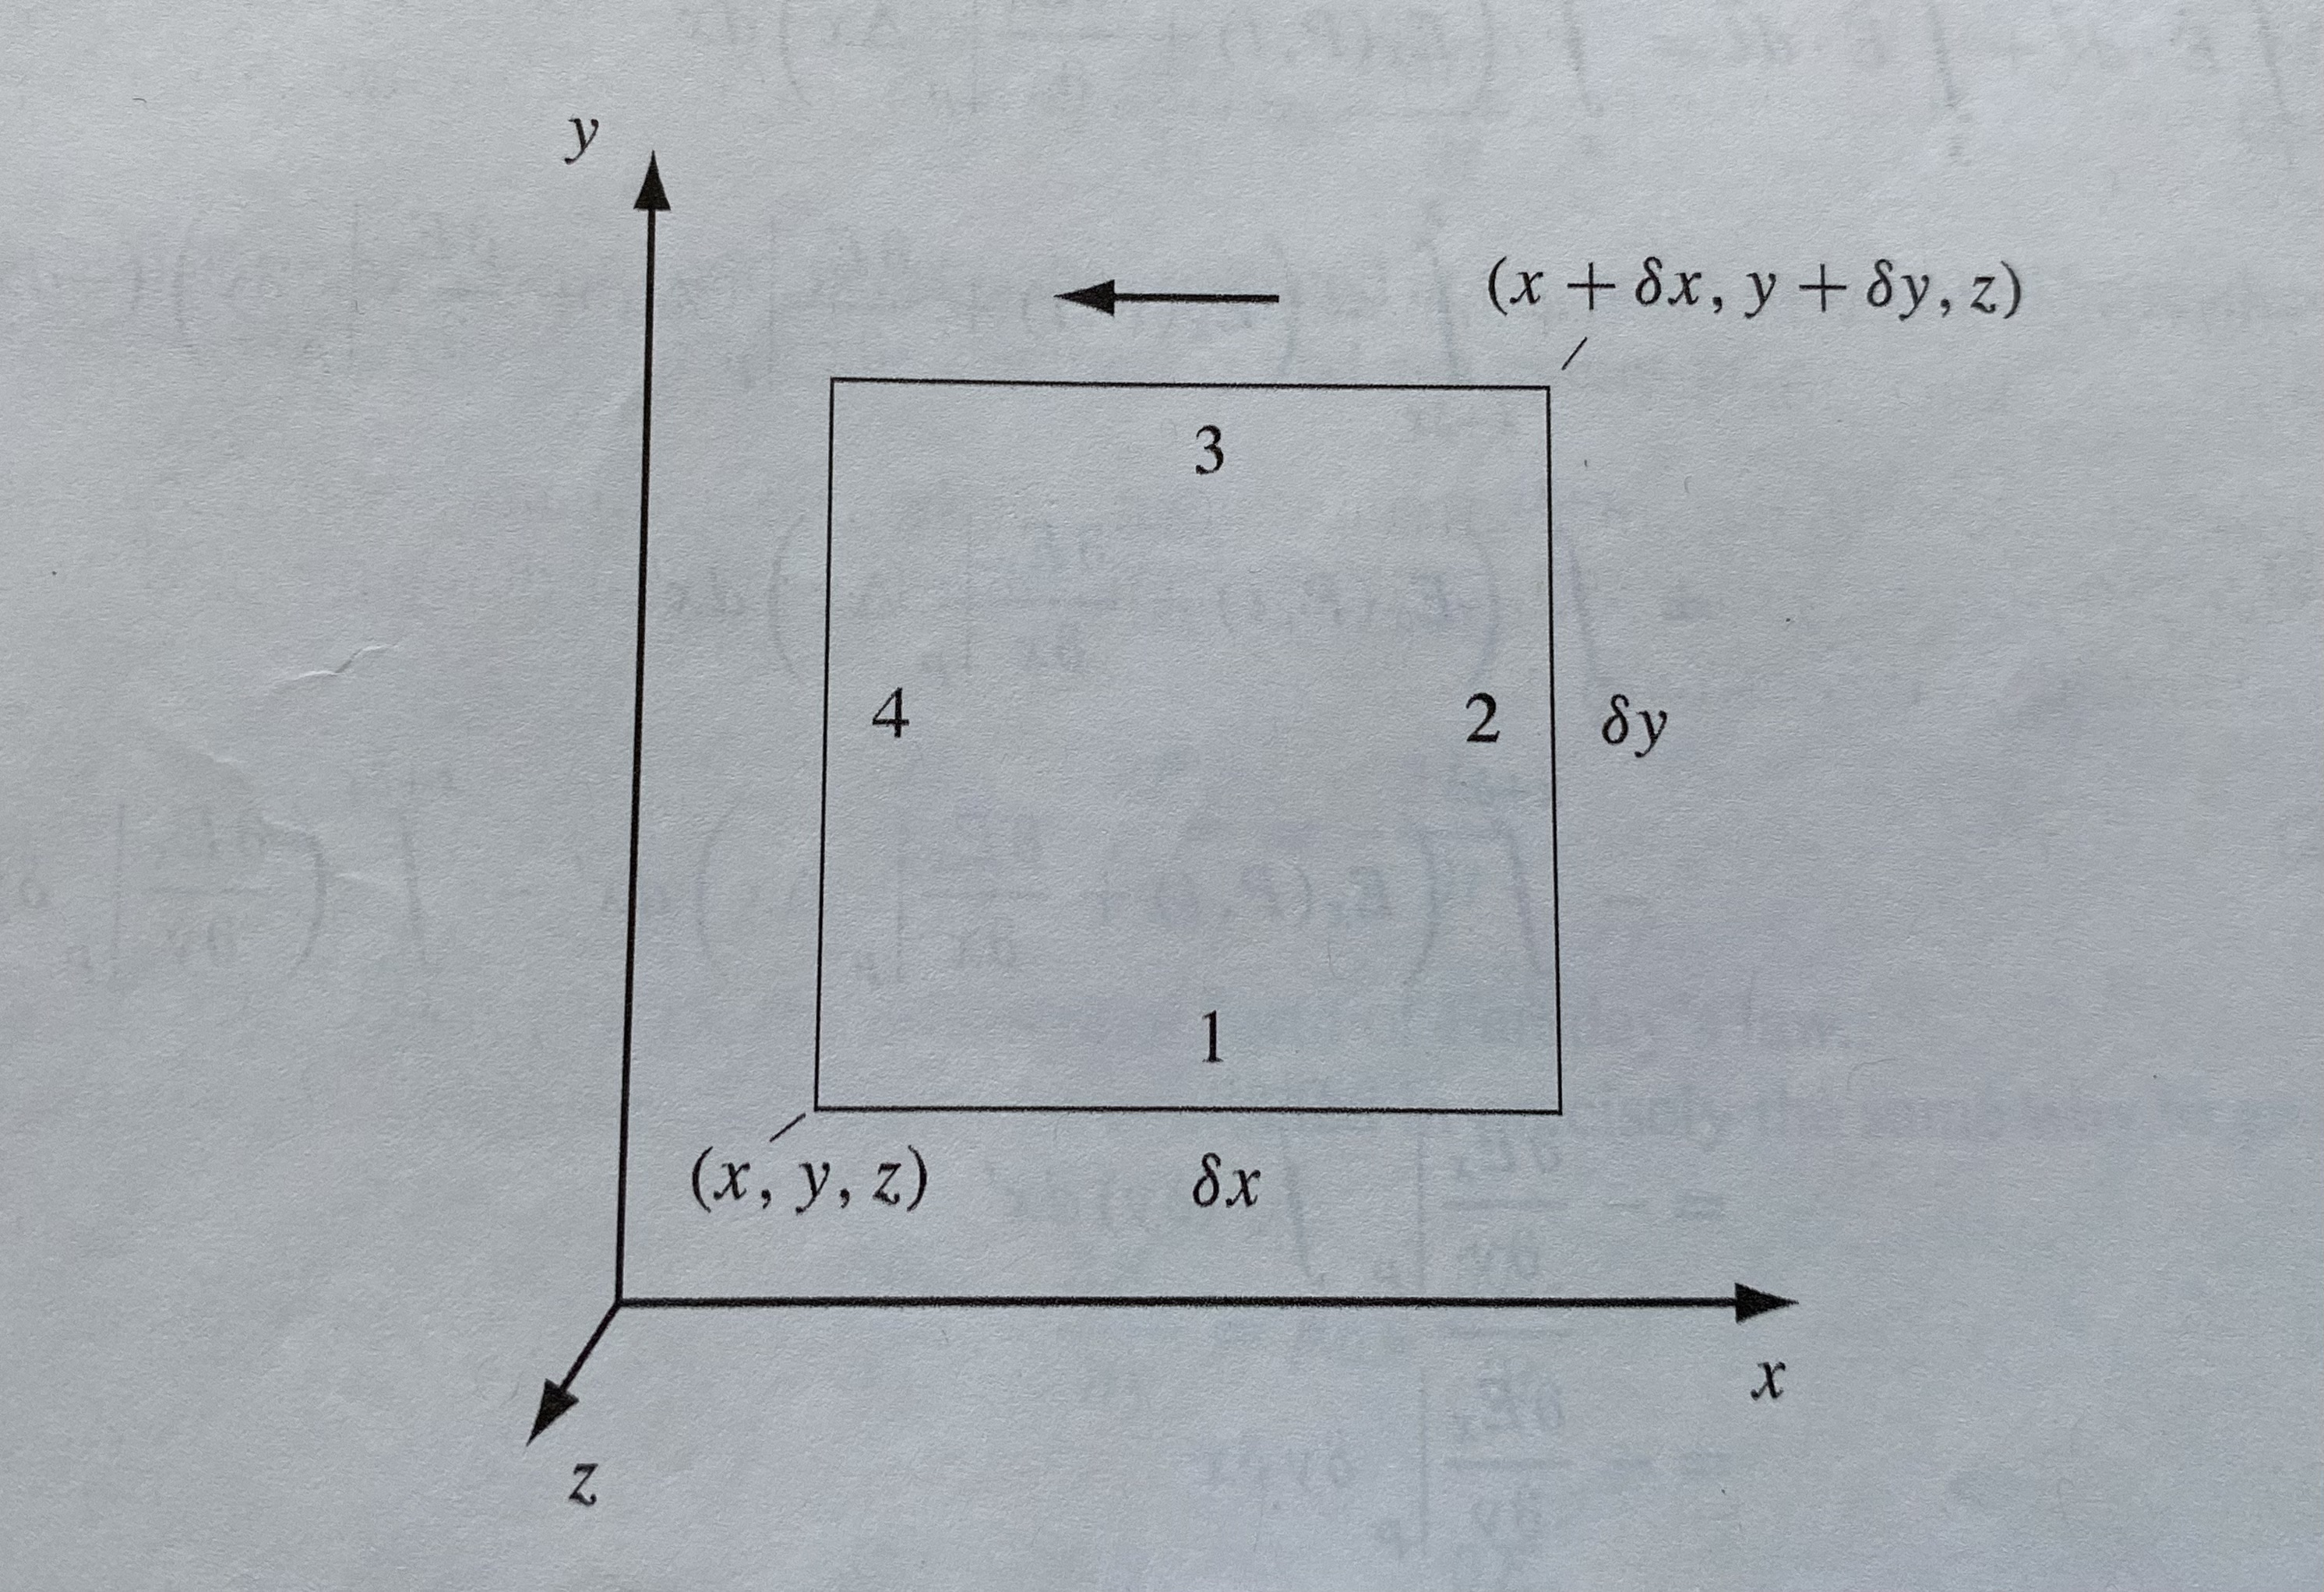
\includegraphics[width=0.8\textwidth]{./pic/IMG_1365.jpeg}
    \centering
    \caption{Path integration in the $x-y$ plane.}
\end{figure}\\
\indent As we proceed around the rectangle, the integrand $\vec{E}\cdot d\,\vec{l}$ selects the component of $\vec{E}$ that is tangent to the curve.\\
\indent To complete the path integration, we use a Taylor series expansion  to express the values of $E_x$ and $E_y$ at all points along the path:
\[
    E_x(\dot{x},\dot{y},\dot{z},t)=E_x(P,t)+\,\frac{\partial{E_x}}{\partial{x}}\Big|_P\,\Delta x+\,\frac{\partial{E_x}}{\partial{y}}\Big|_P\,\Delta y+\,\frac{\partial{E_x}}{\partial{z}}\Big|_P\,\Delta z+\ldots 
\]


\[
    E_y(\dot{x},\dot{y},\dot{z},t)=E_y(P,t)+\,\frac{\partial{E_y}}{\partial{x}}\Big|_P\,\Delta x+\,\frac{\partial{E_y}}{\partial{y}}\Big|_P\,\Delta y+\,\frac{\partial{E_y}}{\partial{z}}\Big|_P\,\Delta z+\ldots 
\]
\\
In these equations, we are expanding each component of the $E_x$ and $E_y$ about the point $P=(x,y,z)$ located
at the lower left corner of the rectangle in Figure. All partial derivatives and the leading term on the right-hand side are evaluated at the single point $P$.\\
\indent We are now in a position to complete the path integration. Begin by breaking the path up into four segments(see Figure).
\[
    \oint \vec{E}\,\cdot\,d\,\vec{l}=\int_1\vec{E}\,\cdot\,d\,\vec{l}+\int_2\vec{E}\,\cdot\,d\,\vec{l}+\int_3\vec{E}\,\cdot\,d\,\vec{l}+\int_4\vec{E}\,\cdot\,d\,\vec{l}
\]
Horizontal segments 1 and 3 involve x-components of $\vec{E}$ that differ only in the value of y.
Along segment 3, $x$ decreases as $l$ increases:
\[
\begin{split}
    \int_1 \vec{E}\,\cdot\,d\,\vec{l}+\int_3 \vec{E}\,\cdot\,d\,\vec{l}=& \int_{x}^{x+\delta x} \Bigl(E_x(P,t)+\,\frac{\partial{E_x}}{\partial{x}}\Big|_P\,\Delta x\Bigl)d\,\dot{x}\\  
    \\
    & +\int_{x+\delta x}^{x}-\Bigl(E_x(P,t)+\frac{\partial{E_x}}{\partial{x}}\Big|_P\,\Delta x+\frac{\partial{E_x}}{\partial{y}}\Big|_P\delta y\Bigl)(-d\,\dot{x})\\
    \\
    =&\int_{x}^{x+\delta x}\Bigl(E_x(P,t)+\frac{\partial{E_x}}{\partial{x}}\Big|_P\,\Delta x\Bigl)d\,\dot{x}\\
    \\
    &-\int_{x}^{x+\delta x}\Bigl(E_x(P,t)+\frac{\partial{E_x}}{\partial{x}}\Big|_P\,\Delta x\Bigl)d\,\dot{x}-\int_{x}^{x+\delta x}\Bigl(\frac{\partial{E_x}}{\partial y}\Big|_P\delta y\Bigl)d\,\dot{x}\\
    \\
    =&-\frac{\partial{E_x}}{\partial{y}}\Big|_P\int_{x}^{x+\delta x}(\delta y)d\,\dot{x}\\
    \\
    =&-\frac{\partial{E_x}}{\partial{y}}\Big|_P\,\delta y \delta x
\end{split}    
\]

Similarly,vertical segment 2 and 4 involve $y-component$ of $\vec{E}$ that differ only in the value of $x$.
\newpage
\[
\begin{split}
    \int_2 \vec{E}\,\cdot\,d\,\vec{l}+\int_4 \vec{E}\,\cdot\,d\,\vec{l}=\int_{y}^{y+\delta y}&\Bigl(E_y+\frac{\partial{E_y}}{\partial{x}}\Big|_P\delta x+\frac{\partial{E_y}}{\partial{y}}\Big|_P \Delta y\Bigl)d\,\dot{y}\\
    &+\int_{y+\delta y}^{y}-\Bigl(E_y+\frac{\partial{E_y}}{\partial{y}}\Big|_P\Delta y\Bigl)(-d\,\dot{y})\\
    =\frac{\partial{E_y}}{\partial{x}}\Big|_P\,&\delta x\delta y
\end{split}
\]
Thus,
\\
\begin{equation}
    \oint \vec{E}\,\cdot\,d\vec{l}=\Bigl(\frac{\partial{E_y}}{\partial{x}}-\frac{\partial{E_x}}{\partial{y}}\Bigl)\Big|_P\,\delta x\delta y\label{A1}
\end{equation}
\indent The right-hand side of Faraday's law involves an integral over the surface enclosed by the path of Figure.
\[
    -\frac{d}{d\,t}\int_A \vec{B}\cdot\,d\,\vec{A}=-\frac{d}{d\,t}\int_A B_z\,d\,A=-\int_A\frac{\partial{B_z}}{\partial{t}}\,d\,A
\]
We assume that the rectangle is sufficiently small so that $\frac{\partial{B_z}}{\partial{t}}$ may be considered constant in the space coordinates $(x,y,z)$.Thus
\begin{equation}
    -\frac{d}{d\,t}\int_A \vec{B}\cdot\,d\,\vec{A}=-\frac{\partial{B_z}}{\partial{t}}\Big|_P\int_A d\,A=-\frac{\partial{B_z}}{\partial{t}}\Big|_P\delta x\,\delta y\label{A2}
\end{equation}
Thus, for the path shown in Figure,Faraday's law \eqref{16} along with Equation \eqref{A1} and \eqref{A2} gives
\begin{equation}
    \frac{\partial{E_y}}{\partial{x}}-\frac{\partial{E_x}}{\partial{y}}=-\frac{\partial{B_z}}{\partial{t}}\label{A3}
\end{equation}
where all derivatives are understood to be evaluated at point(x,y,z).Similarly,the rectangle situated in the $x-z$ and $z-y$ planes give
\begin{equation}
    \frac{\partial{E_x}}{\partial{z}}-\frac{\partial{E_z}}{\partial{x}}=-\frac{\partial{B_y}}{\partial{t}}\label{A4}
\end{equation}

\begin{equation}
    \frac{\partial{E_z}}{\partial{y}}-\frac{\partial{E_y}}{\partial{z}}=-\frac{\partial{B_x}}{\partial{t}}\label{A5}
\end{equation}
\\
Equation \eqref{A3}-\eqref{A5} are the differential form of Faraday's law.\\
\newpage
\indent Ampere's law (Equation \eqref{18}) may be evaluated in precisely the same way to give:
\begin{equation}
    \frac{\partial{B_y}}{\partial{x}}-\frac{\partial{B_x}}{\partial{y}}=\mu_0\,\epsilon\,\,\frac{\partial{E_z}}{\partial{t}}\label{A6}
\end{equation}
\\
\begin{equation}
    \frac{\partial{B_x}}{\partial{z}}-\frac{\partial{B_z}}{\partial{x}}=\mu_0\,\epsilon\,\,\frac{\partial{E_y}}{\partial{t}}\label{A7}
\end{equation}
\\
\begin{equation}
    \frac{\partial{B_z}}{\partial{y}}-\frac{\partial{B_y}}{\partial{z}}=\mu_0\,\epsilon\,\,\frac{\partial{E_x}}{\partial{t}}\label{A8}
\end{equation}
\\
Equation \eqref{A6}-\eqref{A8} are the differential form of Ampere's law.
\newpage
\subsection{Introduction to the surface integration}
To evaluate Gauss's law for electric fields(Equation \eqref{12}),we consider a small cube with sides parallel to each coordinate axis, as shown in Figure. In order to evaluate
the surface integral over the entire cube ,we integrate separately over the six cube faces.\\
\begin{figure}[h]
    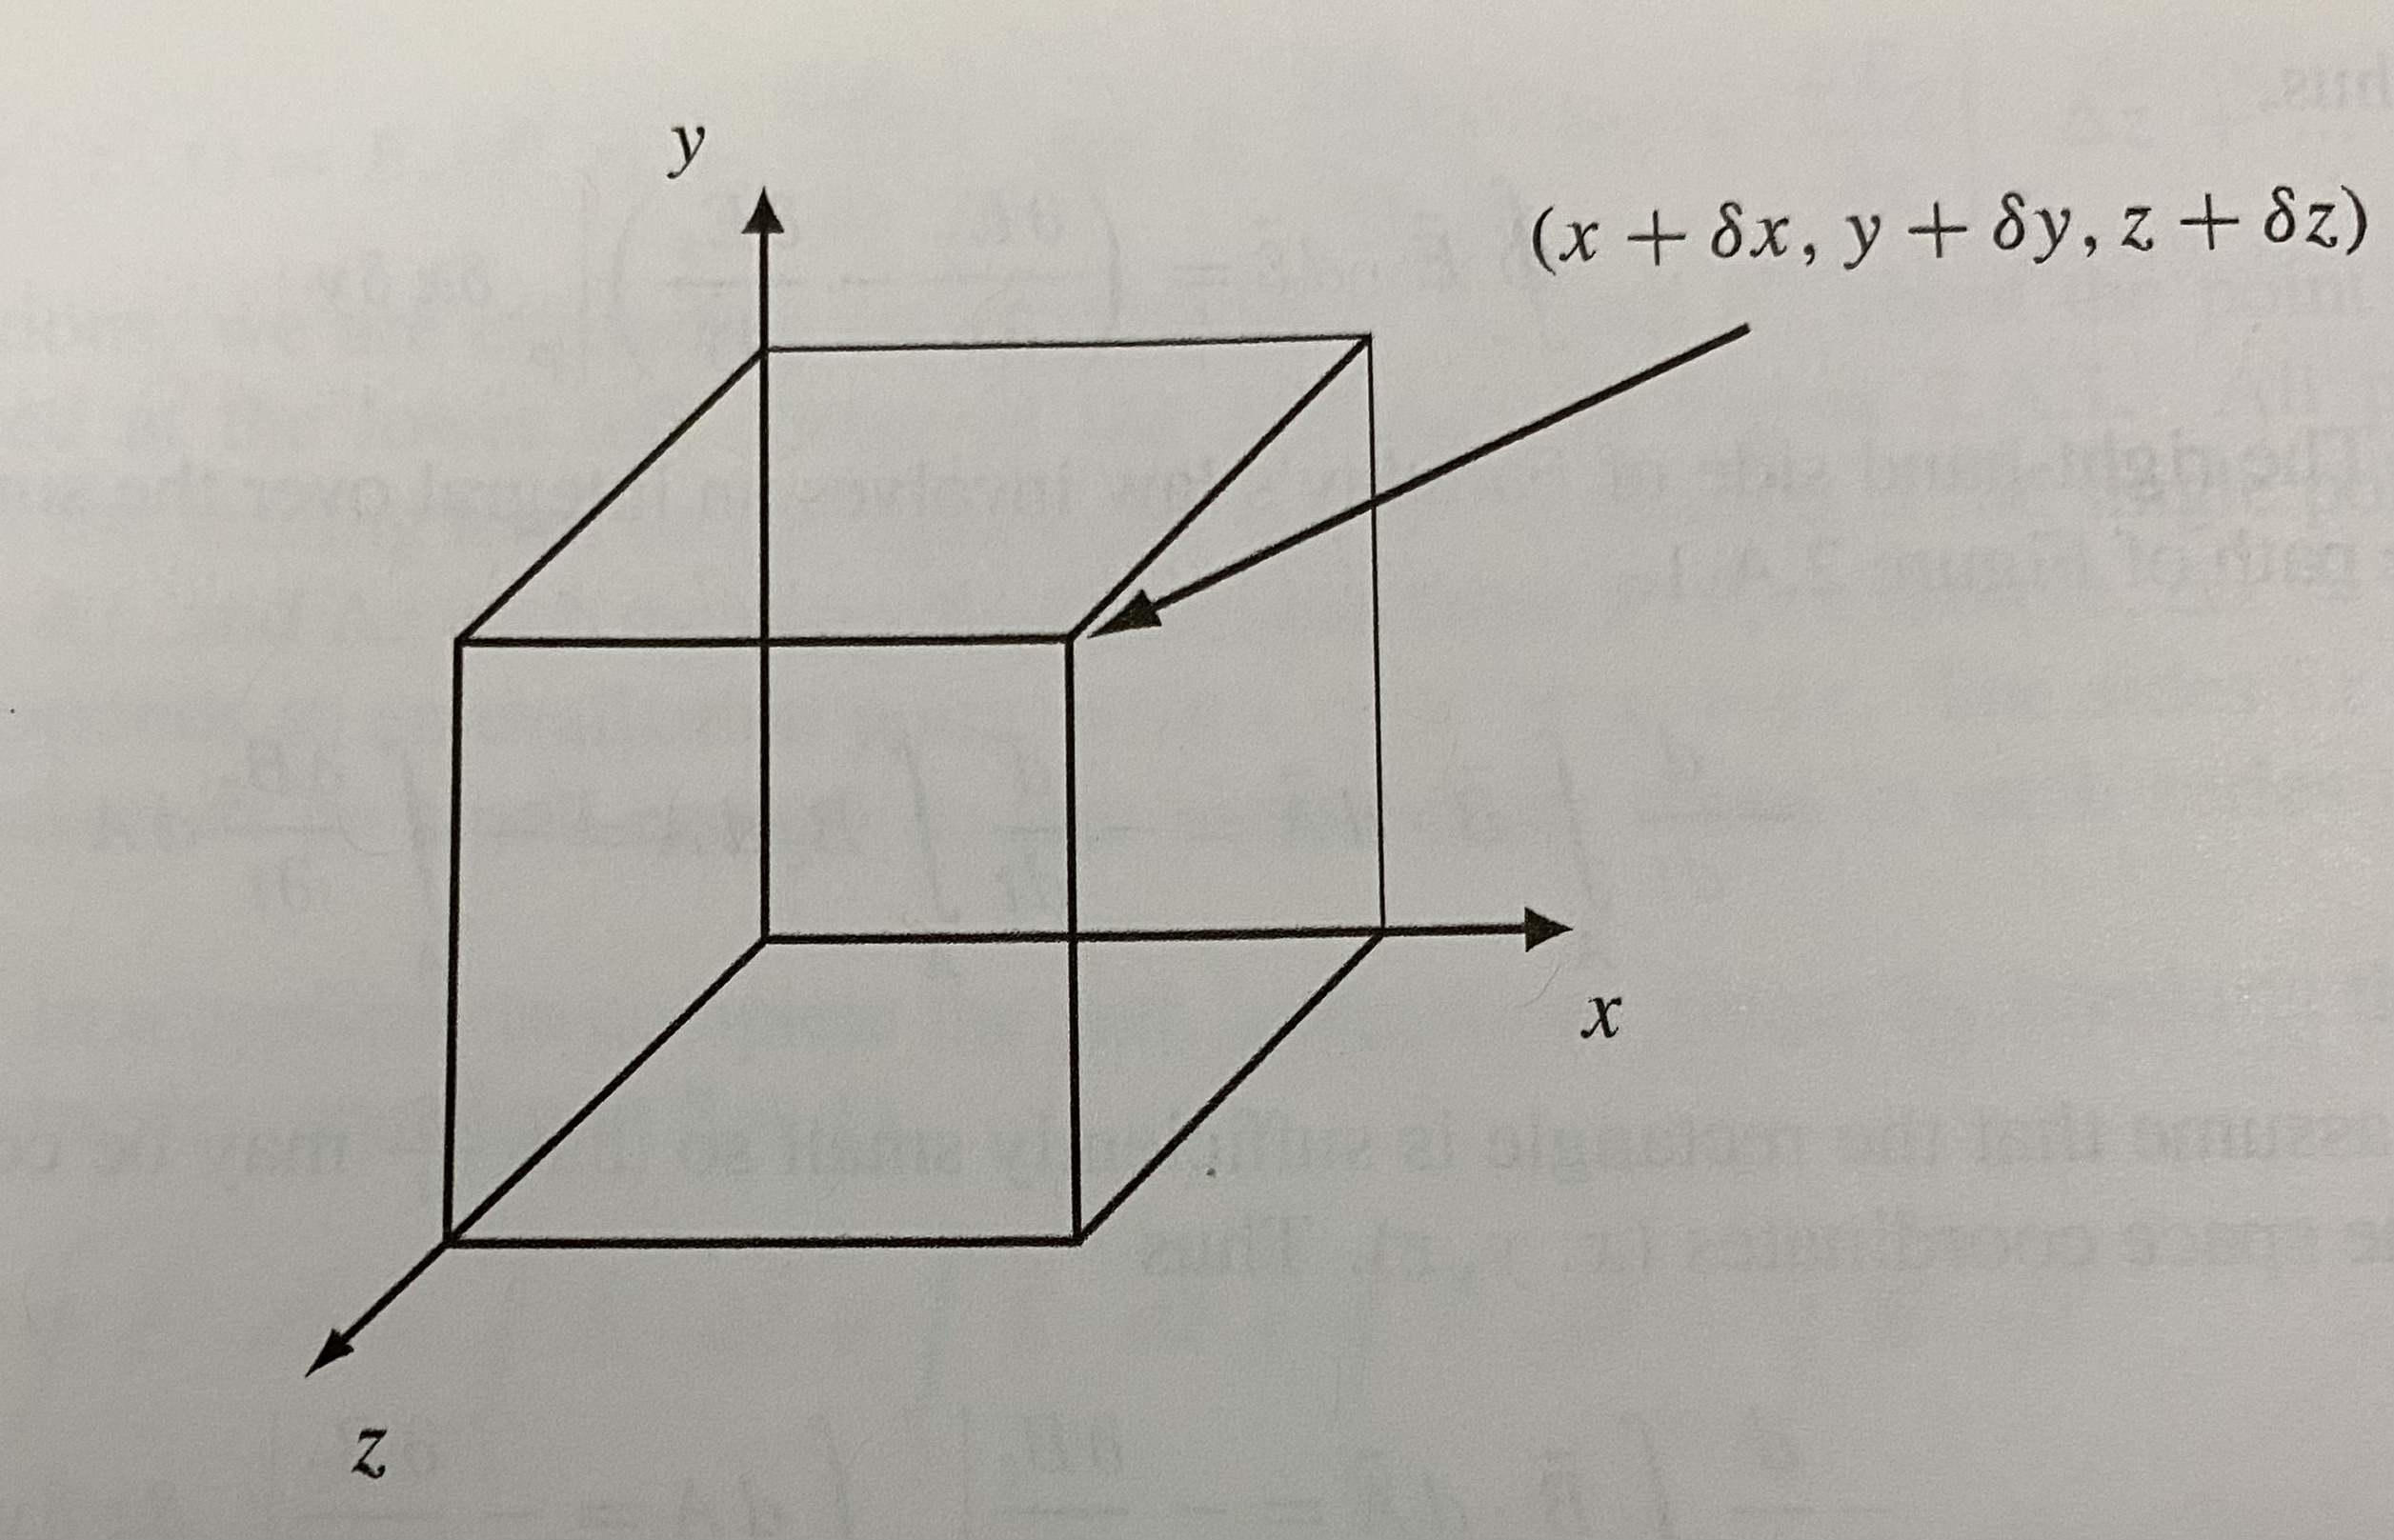
\includegraphics[width=0.6\textwidth]{./pic/IMG_1366.jpeg}
    \centering
    \caption{Surface integration over a cube. The origin of the coordinate axes shown are at $(x,y,z)$, and the corner in the first quadrant is located at $(x+\delta x,y+\delta y,z+\delta z)$}
\end{figure}
\\
\indent Consider the top and bottom surfaces of the cube,located at $y$ and $y+\delta y$.
The direction of $d\,\vec{A}$ over the top surface points along $+y$ and over the bottom surface points in the $-y$ direction.
The contribution to the total electric flux over these two faces can be expressed as follows:
\[
    \begin{split}
        \int_A \vec{A}\cdot d\,\vec{A}=&\int_A E_y(x,y+\delta y,z,t)dx\,dz-\int_A E_y(x,y,z,t)dx\,dz\\
        \\
        =&\int_A \Bigl(E_y(x,y+\delta y,z,t)-E_y(x,y,z,t)\Bigl)dx\,dz\\
        \\
        =&\int_A \biggl(\int_{y}^{y+\delta y}\frac{\partial{E_y}}{\partial{y}}dy\biggl)dx\,dz\\
        \\
        =&\int_V \frac{\partial{E_y}}{\partial{y}}dx\,dy\,dz
    \end{split}
\]
where in the last result,the integration is over the entire volume of the cube. Similar results are obtained over the other two sets of cube faces:
\[
    \oint_A \vec{E}\cdot d\,\vec{A}=\int_V \Bigl(\frac{\partial{E_x}}{\partial{x}}+\frac{\partial{E_y}}{\partial{y}}+\frac{\partial{E_z}}{\partial{z}}\Bigl)dx\,dy\,dz=0
\]
Since the volume is arbitrary, the integrand of the volume integral must be zero.
\begin{equation}
    \frac{\partial{E_x}}{\partial{x}}+\frac{\partial{E_y}}{\partial{y}}+\frac{\partial{E_z}}{\partial{z}}=0\label{A9}
\end{equation}
Equation \eqref{A9} is the differential form of Gauss's law for electric fields.\\
\indent Similar remarks hold for Gauss's law for magnetic fields(Equation \eqref{14}).Thus,
\begin{equation}
    \frac{\partial{B_x}}{\partial{x}}+\frac{\partial{B_y}}{\partial{y}}+\frac{\partial{B_z}}{\partial{z}}=0\label{A10}
\end{equation}
Equation \eqref{A10} is the differential form of Gauss's law for magnetic fields.
\newpage
\subsection{Vector Calculus}
We begin by defining the \emph{gradient operator} in Cartesian coordinates:
\begin{equation}
    \vec{\nabla}=\frac{\partial}{\partial{x}}\hat{i}+\frac{\partial}{\partial{y}}\hat{j}+\frac{\partial}{\partial{z}}\hat{k}
\end{equation}
Using the gradient operator, we may define two new differential operations:the \emph{divergence}
and \emph{curl}. Let $\vec{F}$ represent an arbitrary vector field. The divergence is given by the dot product of $\vec{\nabla}$ and $\vec{F}$.
In Cartesian coordinates,
\begin{equation}
    \begin{split}
        \vec{\nabla}\cdot\vec{F}=&\Bigl(\frac{\partial}{\partial{x}}\hat{i}+\frac{\partial}{\partial{y}}\hat{j}+\frac{\partial}{\partial{z}}\hat{k}\Bigl)\,\cdot\,\Bigl(F_x\hat{i}+F_y\hat{j}+F_z\hat{k}\Bigl)\\
        =&\frac{\partial{F_x}}{\partial{x}}+\frac{\partial{F_y}}{\partial{y}}+\frac{\partial{F_z}}{\partial{z}}
    \end{split}\label{A12}
\end{equation}
The curl is given by the cross product of $\vec{\nabla}$ and $\vec{F}$:
\begin{equation}
    \begin{split}
        \vec{\nabla}\times\vec{F}=
        &\begin{vmatrix}
            \hat{i} &\hat{j} &\hat{k}\\
            \frac{\partial}{\partial{x}} &\frac{\partial}{\partial{x}} &\frac{\partial}{\partial{x}}\\
            F_x &F_y &F_z
        \end{vmatrix}\\
        =&\Bigl(\frac{\partial{F_z}}{\partial{y}}-\frac{\partial{F_y}}{\partial{z}}\Bigl)\hat{i}+\Bigl(\frac{\partial{F_x}}{\partial{z}}-\frac{\partial{F_z}}{\partial{x}}\Bigl)\hat{j}+\Bigl(\frac{\partial{F_y}}{\partial{x}}-\frac{\partial{F_x}}{\partial{y}}\Bigl)\hat{k}
    \end{split}
\end{equation}
\indent These differential operations lead to the following two theorems, stated here without proof: the \emph{divergence theorem} and \emph{Stokes'theorem}.\\
\\
\textbf{Divergence Theorem:} Let $V$ be a volume enclosed by area $A$ and let $\vec{F}$ be a differentiable
vector field. Then 
\begin{equation}
    \int_V \Bigl(\vec{\nabla}\cdot\vec{F}\Bigl)\,d\,\tau=\oint_A \vec{F}\cdot\,d\,\vec{A}
\end{equation}
where in Cartesian coordinates,$d\,\tau=\,dx\,dy\,dz$. The divergence theorem states that the integral of the divergence of a vector field over a region $V$ is determined by the value of the field on the boundary $A$ that encloses the region.\\
\\
\textbf{Stokes' Theorem:} Let the area $A$ be bounded by a curve $C$, and let $\vec{F}$ be a differentiable vector field. Then
\begin{equation}
    \int_A \Bigl(\vec{\nabla}\times\vec{F}\Bigl)\,\cdot\,\,d\,\vec{A}=\oint_C \vec{F}\cdot\,d\,\vec{l}
\end{equation}
Stokes' theorem states that the surface integral of the curl of a vector field is determined by
the magnitude and direction of the vector field on the boundary of the area.\\
\indent We may use the divergence theorem and Stokes' theorem to express Maxwell's equations in differential form.
Begin with Gauss's law for electric fields given by Equation 2.12 and apply the divergence theorem:
\[
    \oint_A \vec{E}\cdot d\,\vec{A}=\int_V \Bigl(\vec{\nabla}\cdot\vec{E}\Bigl)d\,\tau=0
\]
\\
Since the volume $V$ is arbitrary,the integrand of the right-hand side must be zero:
\begin{equation}
    \vec{\nabla}\cdot \,\vec{E}=0
\end{equation}
\\
This is Gauss's law for electric fields (free space) in differential form. IN Cartesian coordinates, it is identical to Equation \eqref{A9}.\\
\indent Similarly,Gauss's law for magnetic fields(Equation 2.13 gives
\[
    \oint_A \vec{B}\cdot d\,\vec{A}=\int_V \Bigl(\vec{\nabla}\cdot\vec{B}\Bigl)d\,\tau=0
\]
\\
As above, this implies
\\
\begin{equation}
    \vec{\nabla}\cdot \,\vec{B}=0
\end{equation}
\\
This is Gauss's law for magnetic fields (free space) in differential form. In Cartesian coordinates, it is identical to Equation \eqref{A10}.\\
\indent For Faraday's law (Equation 2.14) use Stokes' theorem:
\[
    \oint_C \vec{E}\cdot d\vec{l}=\int_A \Bigl(\vec{\nabla}\times\vec{E}\Bigl)\,\cdot\,d\,\vec{A}=-\int_A \frac{\partial{\vec{B}}}{\partial{t}}\,\cdot \,d\,\vec{A}
\]
\\
Since the area $A$ is arbitrary,
\\
\begin{equation}
    \vec{\nabla}\times\vec{E}=-\frac{\partial{\vec{B}}}{\partial{t}}
\end{equation}
\\
This is Faraday's law for free space in differential form. In Cartesian coordinates, it is
equivalent to Equation \eqref{A3} —— \eqref{A5}.\\
\indent Similarly, Ampere's law (Equation 2.15) gives
\[
    \oint_C \vec{B}\cdot d\vec{l}=\int_A \Bigl(\vec{\nabla}\times\vec{B}\Bigl)\,\cdot\,d\,\vec{A}=\mu_0\epsilon\int_A \frac{\partial{\vec{B}}}{\partial{t}}\,\cdot \,d\,\vec{A}
\]
\\
Since the area $A$ is arbitrary,
\\
\begin{equation}
    \vec{\nabla}\times\vec{B}=\mu_0\epsilon\frac{\partial{\vec{E}}}{\partial{t}}
\end{equation}
\\
This is Ampere's law for free space in differential form. In Cartesian coordinates, it is equivalent to Equations \eqref{A6} —— \eqref{A8}.



\end{document}